% flashcards-title: Completed head-to-tail vector addition
% flashcards-desc: Arrows A and B are arranged head-to-tail. Resultant R is a heavier arrow directly from A's original tail to B's final head.
\documentclass[border=5mm]{standalone}
\def\pgfsysdriver{pgfsys-dvisvgm.def}
\usepackage{tikz}
\usetikzlibrary{arrows.meta,calc,patterns.meta,positioning}
\renewcommand{\familydefault}{\sfdefault}

\definecolor{fcInk}{HTML}{1C1C1E}
\definecolor{fcMuted}{HTML}{68686D}
\definecolor{fcGuide}{HTML}{C9C9CE}
\definecolor{fcGold}{HTML}{D7A313}
\definecolor{fcGoldSoft}{HTML}{F8E8AE}

\tikzset{
  fc canvas/.style={fill=white, rounded corners=2.5mm},
  fc vector/.style={
    draw=fcGold,
    line width=1.35mm,
    line cap=round,
    -{Stealth[length=4.1mm,width=3.25mm]}
  },
  fc vector secondary/.style={
    draw=fcInk,
    line width=1.15mm,
    line cap=round,
    dash pattern=on 4.1mm off 2.6mm,
    -{Stealth[length=3.9mm,width=3.1mm]}
  },
  fc resultant/.style={
    draw=fcMuted,
    line width=1.55mm,
    line cap=round,
    -{Stealth[length=4.6mm,width=3.6mm]}
  },
  fc axis/.style={
    draw=fcInk,
    line width=.72mm,
    -{Stealth[length=3.1mm,width=2.5mm]}
  },
  fc guide/.style={
    draw=fcMuted,
    line width=.55mm,
    dash pattern=on 2.3mm off 1.8mm
  },
  fc construction/.style={draw=fcGuide, line width=.32mm},
  fc endpoint/.style={circle, fill=fcInk, inner sep=1.45mm},
  fc label/.style={font=\bfseries\large, text=fcInk},
  fc small label/.style={font=\small, text=fcMuted},
  fc caption/.style={font=\bfseries\small, text=fcMuted}
}

\begin{document}
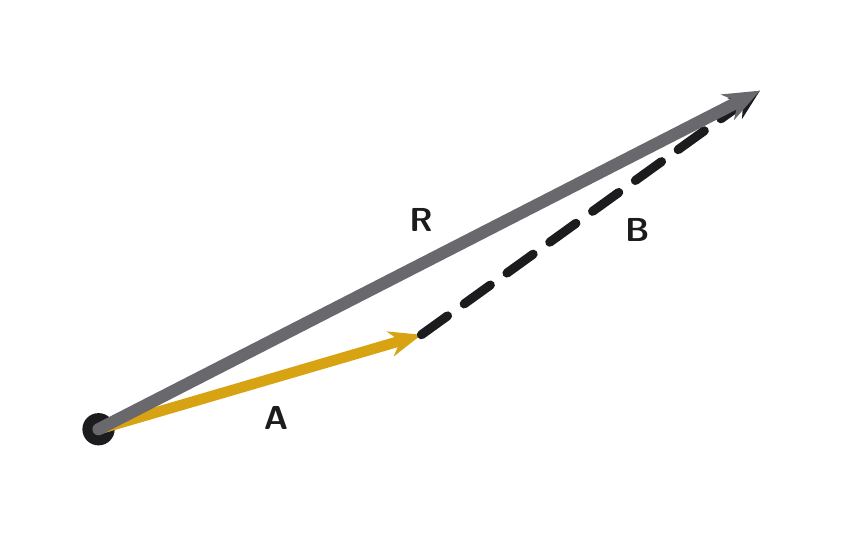
\begin{tikzpicture}[x=1cm,y=1cm]
  \path[fc canvas] (-.35,-.55) rectangle (9.8,5.65);
  \coordinate (O) at (.55,.55);
  \coordinate (M) at (4.65,1.75);
  \coordinate (E) at (8.95,4.85);

  \node[fc endpoint] at (O) {};
  \draw[fc vector] (O) -- (M);
  \draw[fc vector secondary] (M) -- (E);
  \draw[fc resultant] (O) -- (E);
  \node[fc label, below=2.5mm] at ($(O)!.55!(M)$) {A};
  \node[fc label, below right=1mm and 1mm] at ($(M)!.55!(E)$) {B};
  \node[fc label, above left=1.5mm and 0mm] at ($(O)!.52!(E)$) {R};
\end{tikzpicture}
\end{document}
